\section{Layered Architecture}

\begin{figure}[H]
  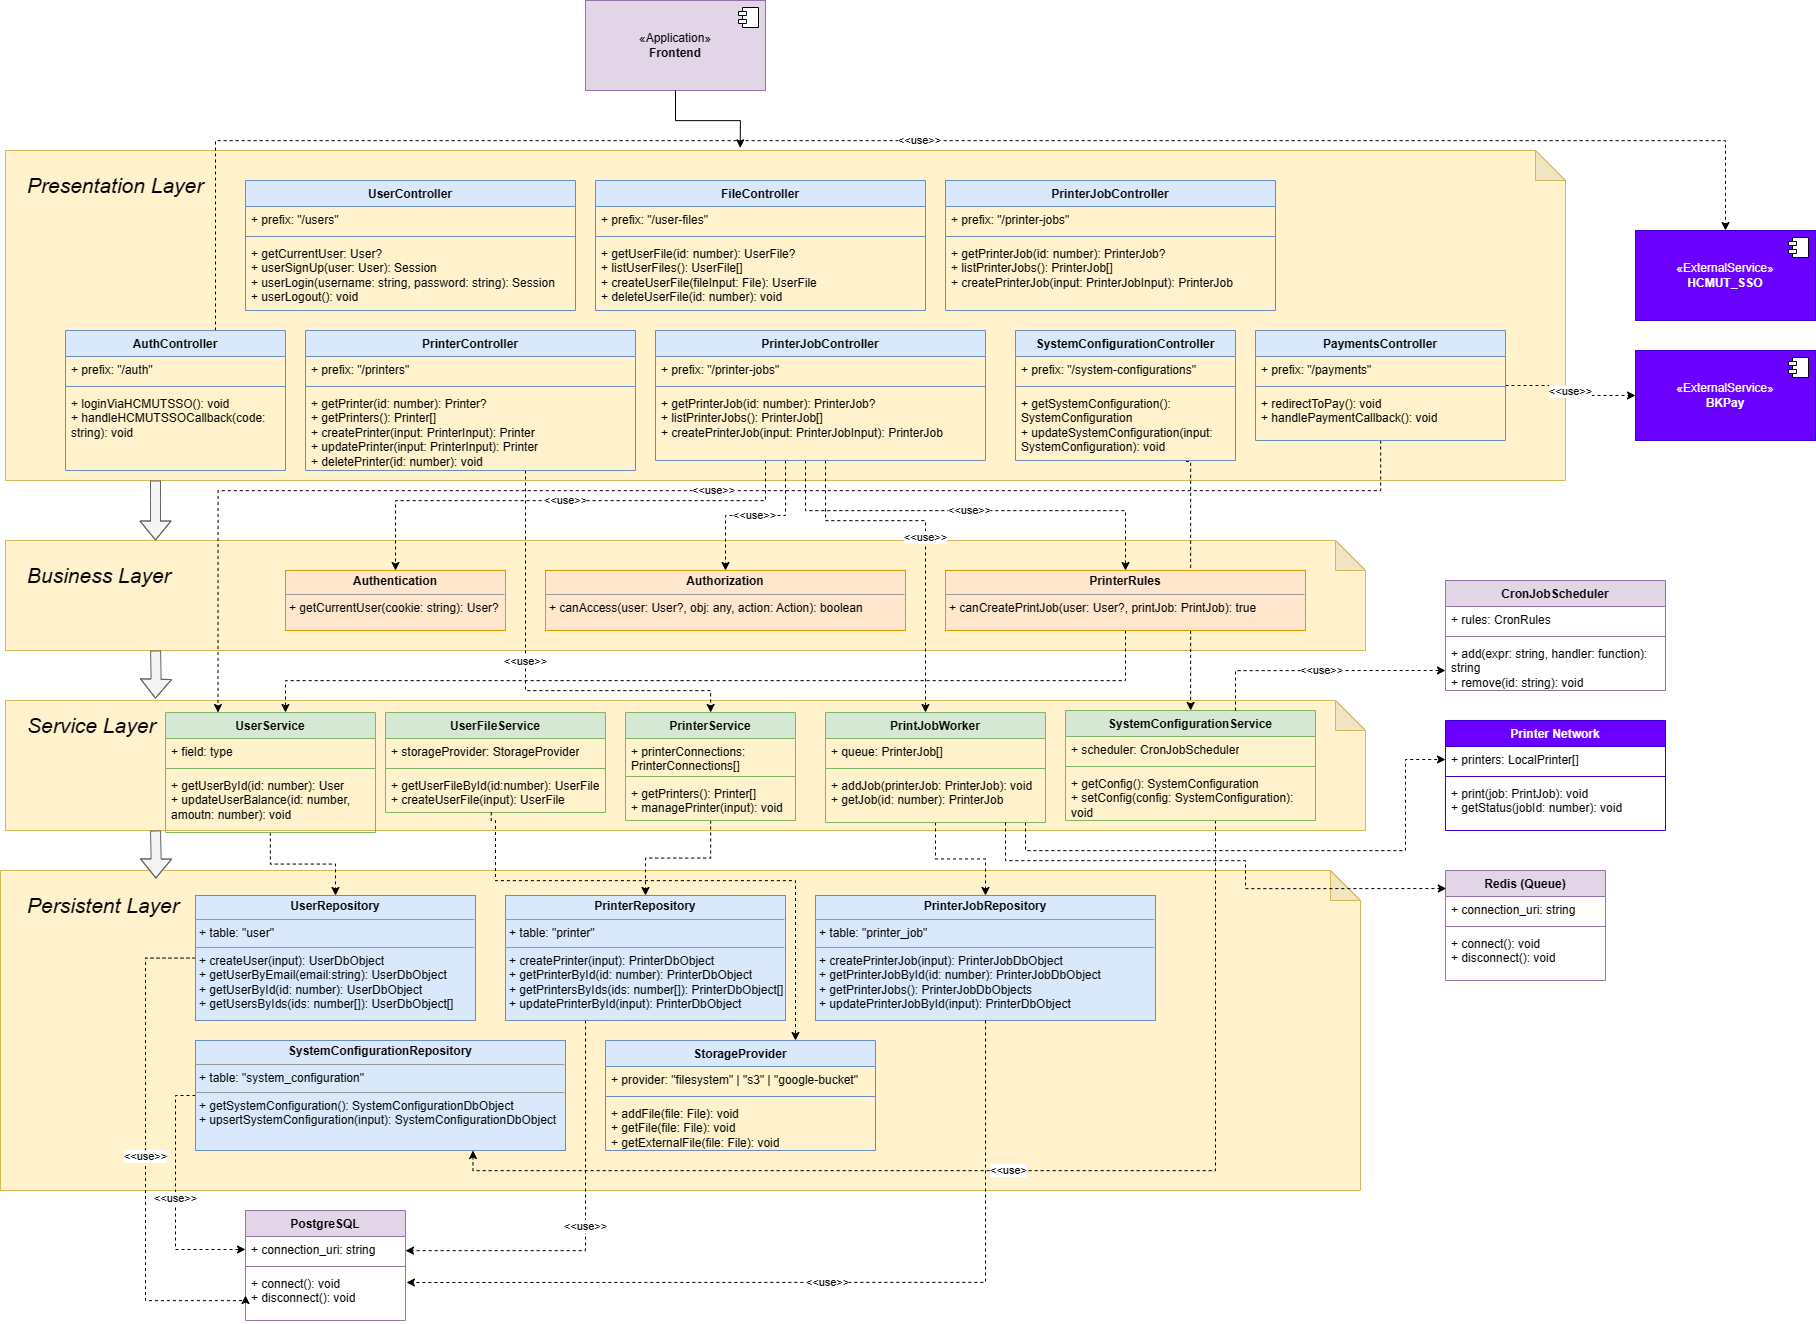
\includegraphics[max height=0.9\linewidth, angle=90,origin=c]{chapters/6. architecture-design/Architecture Diagram.drawio.png}
  \caption{Architecture Diagram}%
\end{figure}

The architecture diagram above demonstrates the layered architecture of our project. It is structured into a four-layer architecture, each serving distinct functions.

In our system architecture, data flow is designed to follow a unidirectional pattern, where each upper layer pulls data from the lower layer, but not vice versa. It somewhat resembles Onion Architecture\footnote{Pal, T. (2021, December 21). Understanding onion architecture. CodeGuru. https://www.codeguru.com/csharp/understanding-onion-architecture/}, whose design principle ensures a clear separation of concerns and enhances system maintainability and scalability. If we do not follow a unidirectional pattern, we can get into some issues like cyclic dependencies (imagine if a presentation component pulls data from a business logic component, but a business logic component in turns pulls data from the presentation component) and coupling.

\subsection{Presentation Layer}

\begin{figure}[H]
  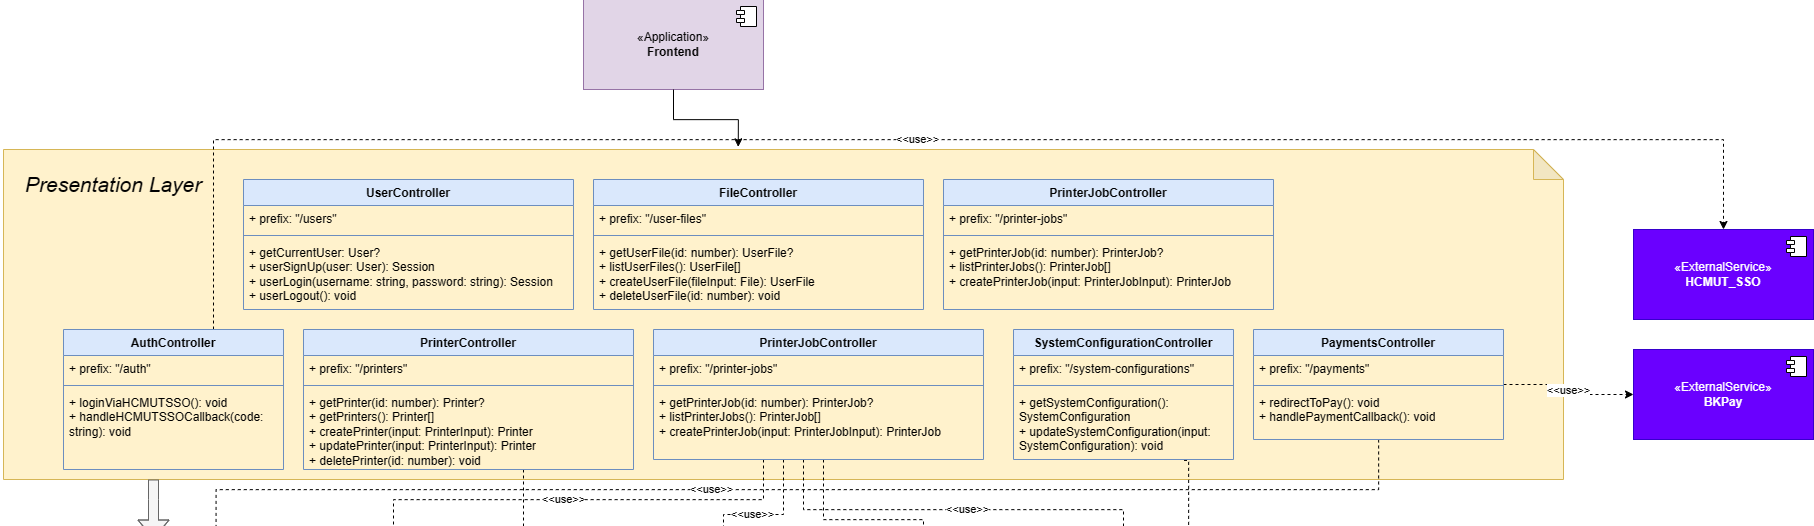
\includegraphics[max width=0.9\linewidth]{chapters/6. architecture-design/Layered Architecture/1. Presentation Layer.png}
  \caption{Presentation Layer}%
\end{figure}

This front-end layer features various controllers for user interaction, handling inputs and outputs for tasks like printing requests, document uploads, and navigating the app. Technically, the components’ interfaces are represented by REST endpoints that get called by the SSPS Mobile App and Web App. The Role of the Controller components are to process the web request by interacting with the service layer to complete the work that needs to be done.\footnote{G, A. (n.d.). Spring MVC Beginner’s Guide. O’Reilly Online Learning. https://www.oreilly.com/library/view/spring-mvc-beginners/9781783284870/ch03s03.html}\\

In our design, before interacting with the application/service layer, we also call onto components of Business Logic Layer to perform checks to ensure that the calling users should be able to call the respective application/service layer operation. For example, the user needs not only to be authenticated (validated using Business layer’s Authentication Service) but they must also be authorized to access the specified resource (validated using Business layer’s Authorization logic) - for example, user should be able to see only their uploaded documents and not anyone else and only admins should be able to make changes to the printer configurations. After receiving the result after calling the application/service layer, the controller layer forms the reasonable response to send back to the client, allowing them to display a UI accordingly to the user.\\

In some cases, the controllers of the presentation layer may also redirect users to some external resources to complete the operation of the lower layer. For example, to login, a controller may redirect the user to HCMUT\_SSO and handle the callback from that service to complete the authentication, or it may redirect the user to BKPAY to complete their page balance purchase. Last, the presentation layer also ensure that the input data is validated and formatted correctly before sending them of to the lower layers.

\subsection{Business Layer}

\begin{figure}[H]
  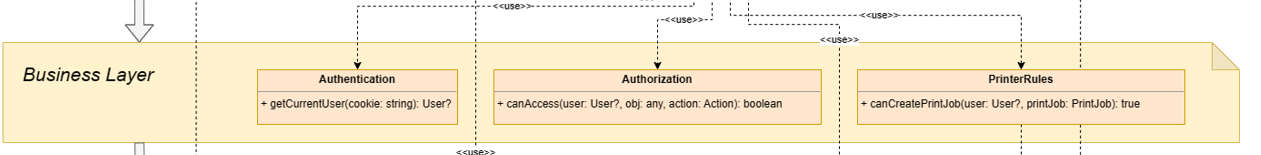
\includegraphics[max width=0.9\linewidth]{chapters/6. architecture-design/Layered Architecture/2. Business Layer.png}
  \caption{Business Layer}%
\end{figure}

Central to the system, this layer manages authentication, authorization, and adherence to printing rules, ensuring that user activities comply with system policies\footnote{Tesha, B. (2020b, March 12). Authentication/authorization is part of the business logic. Medium. https://medium.com/@benedict.tesha/authentication-authorization-is-part-of-the-business-logic-7d6c21627b8e}. The components in this layer are used by the presentation layer for it to make decisions before continuing onto the service layer.\\

To do its role, it must read into some components in the service layer. For example, to check authorization of the user to access a file, it must query the Document Service to determine the file owner to check against the current user. This abstraction is needed because, it should not know the implementation details of how a file is fetched (separation of concern) However, for some components, we may access the persistence layer directly to get the data. For example, for authentication, we query the token of the user from the App Session repository directly. This makes sense because everything authentication-related is handled by the business layer themselves and there is no need to add a corresponding service in the service layer. Separation of service layer and business logic layer is important because it allows the service layer to carry out its role independently. \\

Some components of the application (or internal processes) may call upon other components inside the service layer, in which case we should not need to perform any sort of authentication or authorization check, which is because in this case the caller of these operations is a system, which does not have the user involved. If we couple authentication inside the application, we will end up having to add exceptions to handle these internal use cases and would end up with an unmaintainable codebase. \\

Having a business layer before requests get routed to the service layer is obviously to ensure security and policy of the system and to make sense of business requirements like page balance.

\subsection{Service Layer}

\begin{figure}[H]
  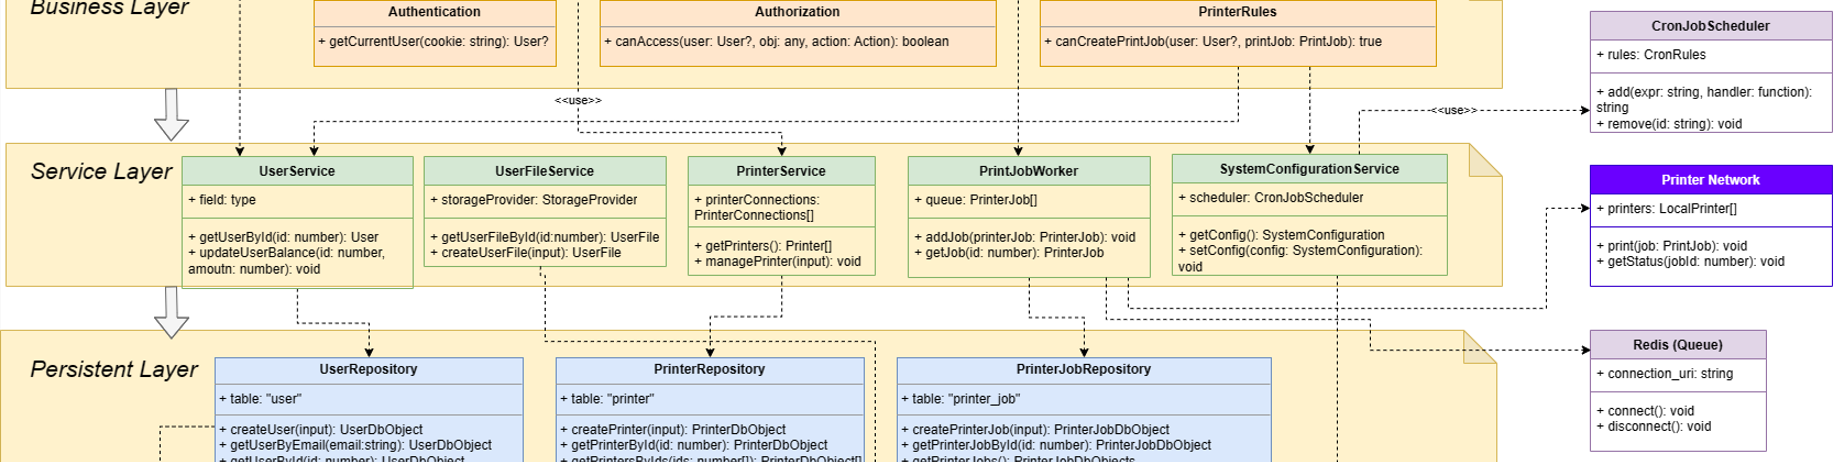
\includegraphics[max width=0.9\linewidth]{chapters/6. architecture-design/Layered Architecture/3. Service Layer.png}
  \caption{Service Layer}%
\end{figure}

Here, specialized services operate, including User Service for managing user information and balance, User File Service  for document and upload management, Payment Service for financial transactions, Printer Service for printer management and communication, Report Generator for creating reports, and Print Job Queue for organizing print jobs. The service layer / service layer centralizes logic to perform various tasks in the application. These logic is often organized into reusable modules for use by different aspects of the system, which allows the codebase to much more maintainable\footnote{Bedmutha, A. (2023, June 6). Why do we need Service layers? - Apoorv Bedmutha - Medium. Medium. https://medium.com/@bedmuthaapoorv/why-do-we-need-service-layers-ecf86ca5c739}.\\

In the case where other components of the system call another service, it is ideal because these other components must not know about implementation details of that service (how the data is fetched, written). This abstraction is helpful because along the way, the implementation detail of that service may change, but its public API remains the same, allowing other use cases to carry out as usual without having to make changes to accommodate.\\

Organizing logic into different services inside the application layer also makes it easier to manage and understand the dependencies between various services, which is important to ensure data requirement and flow are compatible.\footnote{ Parker, J. (2023, April 2). What is service layer in software architecture? - Architecture. Design Your World - Explore Architecture. https://www.architecturemaker.com/what-is-service-layer-in-software-architecture}. This organization is also particularly important in service-oriented architectures where services are shared and categorized into different layers.

\subsection{Persistent Layer}

\begin{figure}[H]
  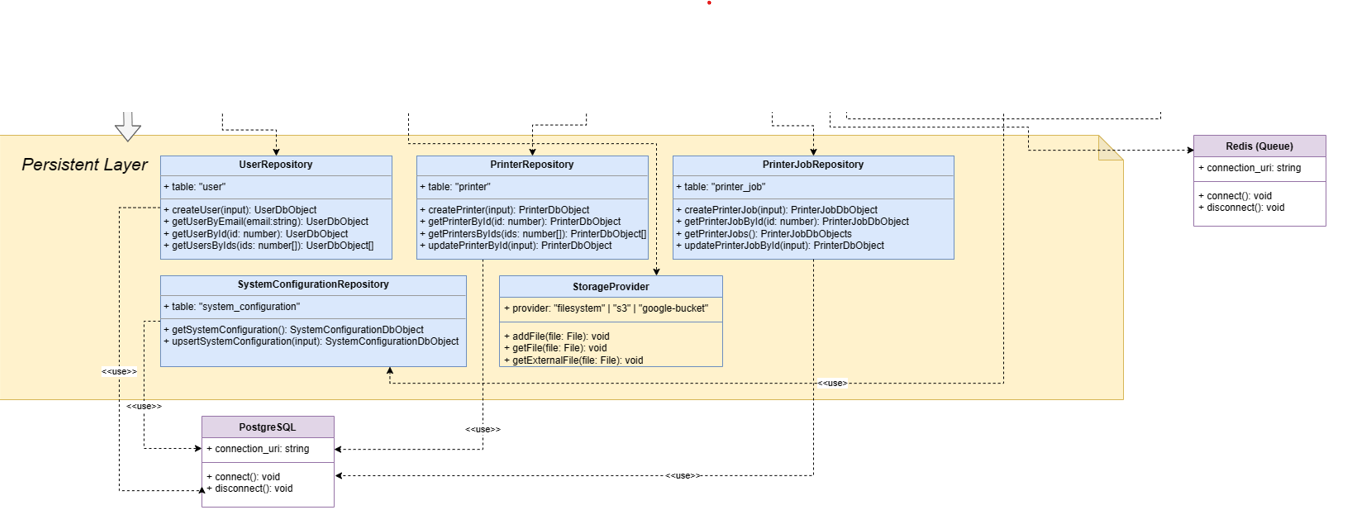
\includegraphics[max width=0.9\linewidth]{chapters/6. architecture-design/Layered Architecture/4. Persistent Layer.png}
  \caption{Persistent Layer}%
\end{figure}

Acting as an intermediary between the Service and underlying data provider, this layer consists of repositories for consistent and secure data transactions. They are abstractions to manage data storage and retrieval processes (operations to save, update, delete and query data). The abstraction of data source is helpful because it allows changes in the data storage without impacting the higher layer. For example, along the way, we might change from PostgreSQL to use a non-SQL database like MongoDB. This change does not require any changes from service code of the upper level because the repository class still maintains the same public APIs (eg. getUserById, getPrintingHistoryByUserId) as well as Data object (UserDbObject, PrinterDbObject). \\

In addition, this layer also ensures data integrity and security by enforcing validation rules and maintaining consistency across databases, which can be achieved by the abstraction of Database Object classes that perform validation upon initialization. Similarly, by removing the need for the upper layer to write database queries directly (given how different databases might have different syntax), we make the upper layer’s code more maintainable and more resilient against changes in the infrastructure (database system component for specific)\footnote{Jamesmontemagno. (2023, February 21). Designing the infrastructure persistence layer - .NET. Microsoft Learn. https://learn.microsoft.com/en-us/dotnet/architecture/microservices/microservice-ddd-cqrs-patterns/infrastructure-persistence-layer-design
}.\\

\section{Component diagrams}
\subsection{Printing Service}
\begin{figure}[H]
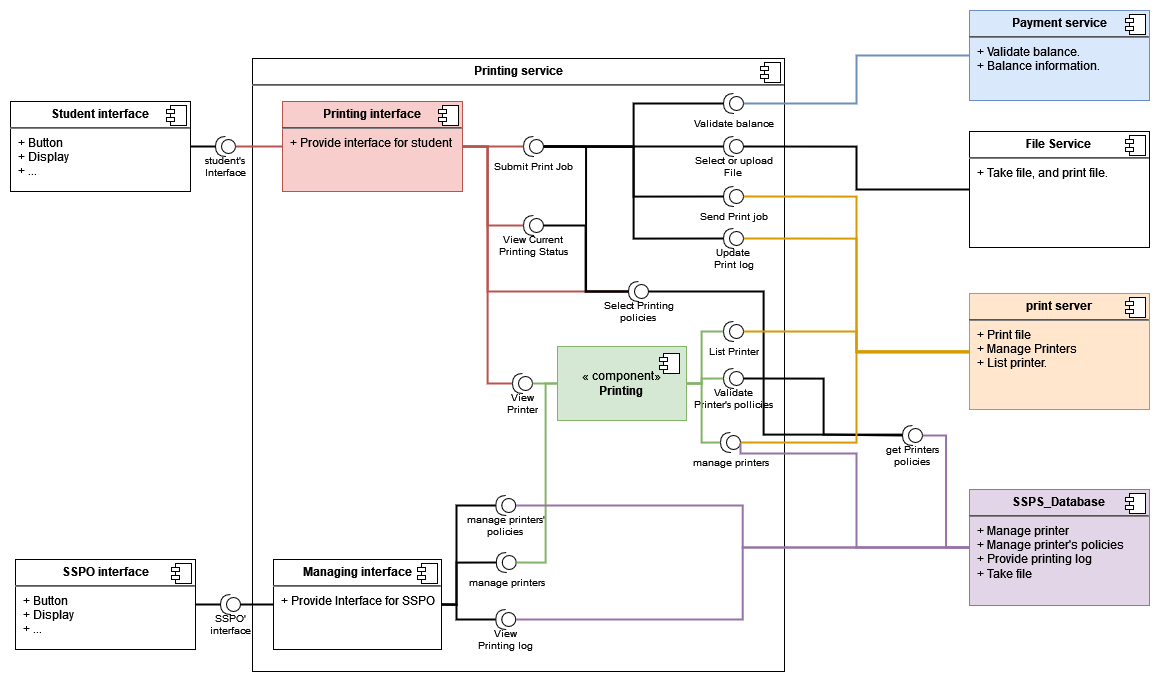
\includegraphics[max width = 0.9\linewidth,origin = c]{chapters/6. architecture-design/Component Diagram/printing.png}
  \caption{Printing service}%
  \end{figure}

This diagram represents the architecture of the printing service system, which is composed of five main components, each with distinct functionalities: 
\begin {enumerate}
    \item \textbf{Managing and Printing Interfaces:} These interfaces are crucial for interaction, designed to handle and efficiently respond to inputs from both students and the Student Services and Programs Office (SSPO). They enable a user-friendly experience for managing print jobs and provide real-time feedback.
    \item \textbf{Printer Manager:} A vital component that facilitates communication with the print server. It's responsible for the operational aspects of printing, including queue management, printer status monitoring, and error handling. This manager ensures that the printing process is smooth and efficient.
    
\end{enumerate}
    Beside main components in the service, the printing service also provide some interfaces from other components and services. This also show the relationships between service are important. \\
\subsection{Payment service}
\begin{figure}[H]
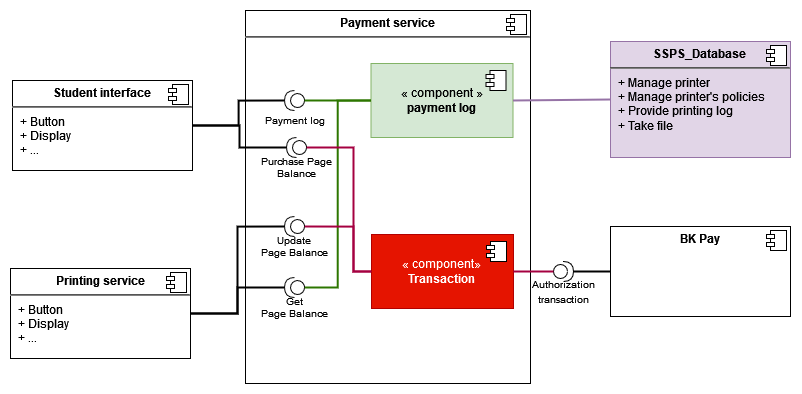
\includegraphics[max width = 0.9\linewidth,origin = c]{chapters/6. architecture-design/Component Diagram/payment.png}
  \caption{Payment service}%
  \end{figure}
Expanding on the Payment Service, it includes two main components with specific roles:
\begin{enumerate}
    \item \textbf{Payment Log:} This component is dedicated to recording and maintaining a comprehensive log of all payment transactions. It is essential for tracking payment histories, verifying transactions, and providing users and administrators with detailed financial reports.
    \item \textbf{Transaction:} It focuses on managing the actual transaction processes. This includes handling various payment methods, securing transaction data, and ensuring the efficient processing of user payments. It is designed to be robust and secure, capable of handling high volumes of transactions with accuracy.
\end{enumerate}
This service also extends its functionalities to the printing service, offering integration methods that allow for seamless financial transactions within the printing system.



\subsection{User Authentication service and reporting service}
\begin{figure}[H]
    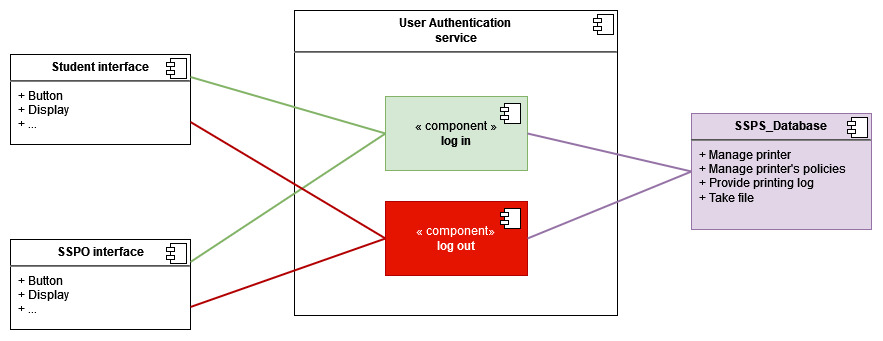
\includegraphics[max width = 0.9\linewidth,origin = c]{chapters/6. architecture-design/Component Diagram/Login.jpg}
    \caption{User Authentication service}%
\end{figure}

\begin{figure}[H]
    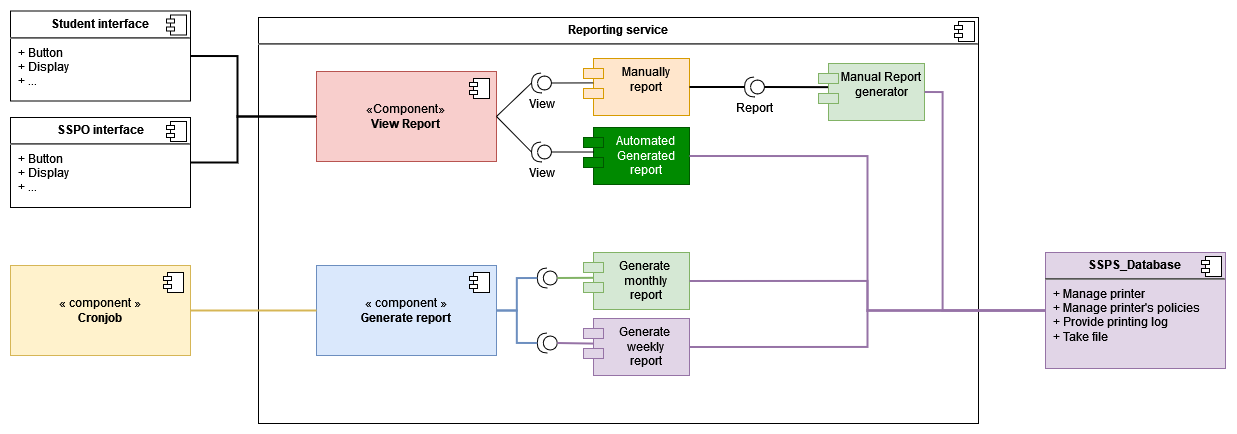
\includegraphics[max width = 0.9\linewidth,origin = c]{chapters/6. architecture-design/Component Diagram/report.png}
    \caption{Reporting service}%
\end{figure}
Lastly, the system encompasses additional modules, such as:
\begin{enumerate}
    \item \textbf{User Authentication Service:} This module is responsible for securing the system by managing user logins and logouts. It employs robust security protocols to ensure user identity verification, access control, and data protection.
    \item \textbf{Reporting Service:} This service is designed to compile and provide comprehensive reports on various aspects, such as usage statistics, operational performance, and financial summaries. It can generate weekly or monthly reports, offering valuable insights for management and decision-making processes.
\end{enumerate}
These services not only enhance the overall system functionality but also ensure operational integrity and user satisfaction.